\documentclass{article}

\usepackage{packages}
\usepackage{environments}
\usepackage{commands}

\begin{document}

\title{Typing Analysis}
\author{Dima Trushin}
\date{}
	
\maketitle
\tableofcontents

\section{General information}

The application uses Qt environment as an ecosystem. It does not use RTTI but uses exceptions. All components of the program must be inside NSApplication namespace. Nested namespaces should be placed in a subfolder of the project.

\subsection{Addressable objects}

I use term addressable object. It means an object that can be referenced by other objects. There are several types of addressable objects:
\begin{enumerate}
\item QObject
\item CApplicationImpl
\item Observer/Observable (TO DO)
\end{enumerate}
Addressable objects must be created on heap via \verb"std::make_unique" or similar mechanism. An exception to this rule: you may create an addressable object inside another addressable object.

\subsection{Exceptions}

The strategy is to catch exception, show a message, and die. Since Qt environment is not totally exception safe, it is not allowed to throw exceptions in an event loop. If a QObject requires to throw an exception and terminate the program it catches the exception by itself and then sends a signal to CQtLoopException object. CQtLoopException shows a message and stops the event loop. CQtLoopException is a singleton, it uses CAnyGlobalAccess template (see~\ref{section::Singleton}).

\section{Application Structure}

\subsection{Overview}

CApplication object initialize all required resources for the application including the ones to interact with Qt ecosystem. It may throw an exception while constructing. In order to minimize stack usage CApplication contains \verb"std::unique_ptr" to CApplicationImpl (it is addressable object). CApplicationImpl consists of four parts:
\begin{enumerate}
\item \textbf{CApplicationGlobals}. Its purpose is to initialize global resources, e.g., timers, loggers, thread pools, etc. Application initializes all global resources (basically singletons) at the start. This allows not to wast time on the first call. Also, it is inconvenient to initialize timers via the first call.
\item \textbf{CApplicationKernel}. Its purpose is to initialize the kernel of the application. The kernel does not depend on the GUI and uses MVC via observer pattern to interact with GUI.
\item \textbf{CApplicationGUI}. Its purpose is to provide View wrappers over Qt resources compatible with MVC pattern.
\item \textbf{CApplicationImpl}. Its purpose is to connect the kernel and the GUI via MVC.
\end{enumerate}
The order of construction is ensured by the inheritance mechanism.
\begin{center}
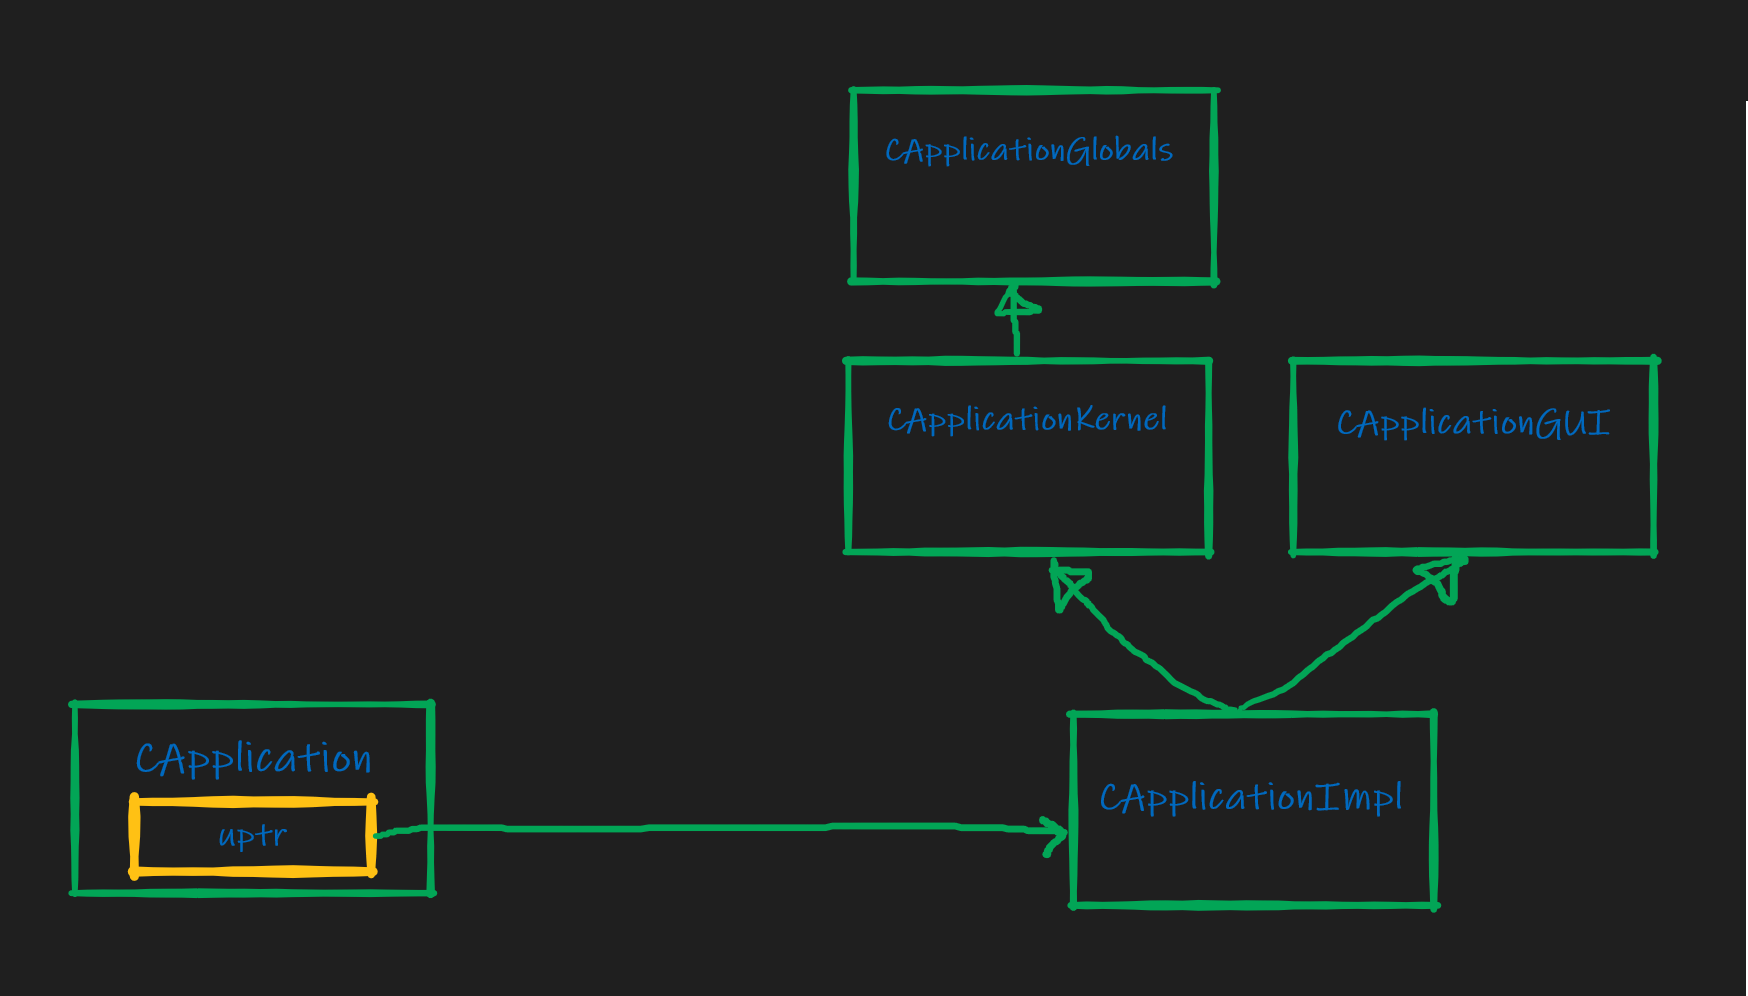
\includegraphics[scale = 0.3]{Figures/CApplicationStructure.png}
\end{center}

\subsection{Global Objects}

\paragraph{Timer}

Application uses one main timer. This is a singleton with respect to the template here~\ref{section::Singleton}. It starts in the constructor of CApplicationGlobal. Timer return CTime object. It does not depend on particular units but you may convert it to any units you want. Internally \verb"std::chrono" is used.

\subsection{Kernel}

\subsection{Qt Resources}

\subsection{ApplicationImpl}


\section{Code}

\section{Implementation}

\section{Library}
\subsection{Singleton}\label{section::Singleton}
CAnyGlobalAccess template consists of three parts:
\begin{enumerate}
\item \textbf{CAnyGlobalAccessible}. It provides a static storage for a global object. You do not access it directly.
\item \textbf{CAnyGlobalAccess}. This object is used to access the global object. The global object must be initialized before access object is created.
\item \textbf{CAnyGlobalInitializer}. This object is used to initialize the global object. You need to create one instance of this object in order to initialize the global object.
\end{enumerate}
\begin{center}
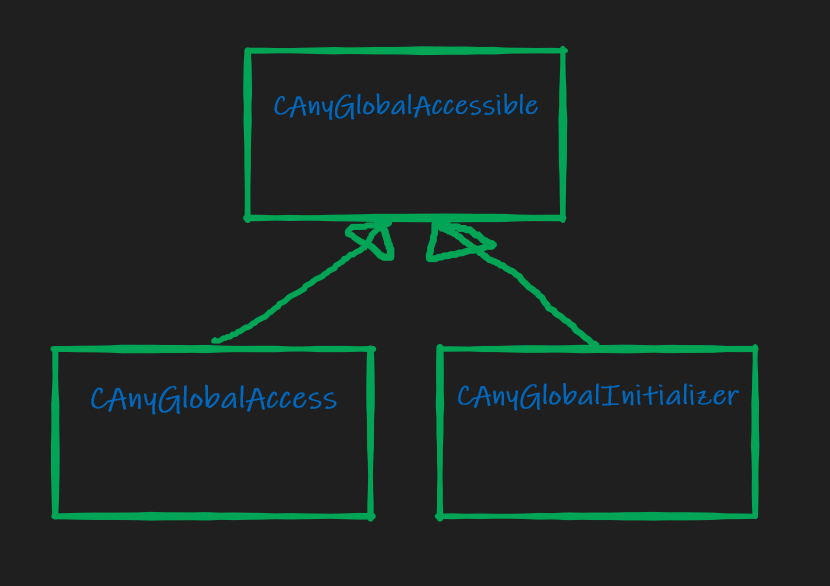
\includegraphics[scale = 0.3]{Figures/CAnyGlobalAccess.png}
\end{center}

\paragraph{Description}
The pattern is used to make a global object with non-trivial constructor without explicitly defining the object globally. \textbf{WARNING} this thing is NOT thread safe! In order to use the pattern we must provide:
\begin{enumerate}
\item \verb"TAccessible" -- the class for the global object

\item \verb"TID" -- identification class. If we want to have several global objects  of a class Type, we must distinguish them by a dummy class \verb"TID". For example, \verb"CAnyGlobalAccessible<Type, A>" and \verb"CAnyGlobalAccessible<Type, B>" store  different instances of objects of type Type in static storage. Since static objects defined by the class they belong to, classes \verb"A" and \verb"B" are required to distinguish the instances.

Example of a dummy class declaration:
\begin{verbatim}
class CGlobalAccessibleID;
\end{verbatim}

\item A class for initialization of the global object. It must be
 inherited from \verb"CAnyGlobalInitializer". The class must inherit all the constructors of the base class.
\begin{verbatim}
class CMyInitializer : CAnyGlobalInitializer<TAccessible, TID> {
   using CBase = CAnyGlobalInitializer<TAccessible, TID>;
 public:
   using CBase::CBase;
 };
\end{verbatim}

\item A class for getting access to the global object must be publicly inherited from \verb"CAnyGlobalAccess". It has only a default constructor. It asserts if  the global object has not yet been initialized.
\begin{verbatim}
class CMyAccessor : public CAnyGlobalAccess<TAccessible, TID> {};
 \end{verbatim}
\end{enumerate}

\paragraph{Example}
Suppose we want a global \verb"int" variable for logging:
\begin{verbatim}
class CLoggerCounterID;
class CLoggerCounterInitializer :
  CAnyGlobalInitializer<int, CLoggerCounterID> {
  using CBase = CAnyGlobalInitializer<int, CLoggerCounterID>;
public:
  using CBase::CBase;
};
class CLoggerCounterAccess : public CAnyGlobalAccess<int, CLoggerCounterID> {};
\end{verbatim}
Then in code we write something like that:
\begin{verbatim}
...
CLoggerCounterInitializer Init(0);
...
CLoggerCounterAccess LogCounter;
++(*LogCounter);
std::cout << *LogCounter << std::endl;
...
\end{verbatim}
\end{document}
